%&"../mdl"
\endofdump
\tikzexternalize[prefix=cache/]{hw1}
\begin{document}
    \title{作业一:MLQP}
    \maketitle

    \section{推导}
    \begin{problem}
        Suppose the output of each neuron in a multi-
layer perceptron is:

\begin{equation}\label{eq:def}
    x_{kj} = f\left(\sum_{i=1}^{N_{k-1}}(u_{kji}x_{k-1,i}^2+v_{kji}x_{k-1,i})+b_{kj}\right)
\end{equation}

where both $u_{kji}$ and $v_{kji}$ are the weights connecting the $i^\text{th}$ unit in the layer $k-1$ to the $j^\text{th}$ unit in the layer $k\in[2,M]$, $b_{kj}$ is 
the bias of the $j^\text{th}$ unit in the layer $k\in[2,M]$, $N_k$ is the number of 
units  if $1\leq k\leq M$ and $f(\cdot)$ is the sigmoidal activation 
function. 

Please derive a back-propagation algorithm for multilayer 
quadratic perceptron (MLQP) in on-line or sequential 
mode.
    \end{problem}

    \begin{figure}[h]
        \centering
        
\includegraphics[height=0.25\textheight]{mlqp}
        \caption{MLQP}\label{fig:mlqp}
    \end{figure}

    \subsection{输出神经元}
        对于输出神经元信号 $x_{Mj}$ 来说,令 $d_{Mj}$ 为目标值,则对应的误差为
        \begin{equation*}
            e_{Mj} = d_{Mj} - x_{Mj}
        \end{equation*}
        % 如果效果不理想,将会采用交叉熵函数。
        使用均方误差计算损失函数
        \begin{equation}\label{eq:loss}
            \mathcal{E} = \sum_{j=1}^{N_{M}}\frac{1}{2}e_{Mj}^2
        \end{equation}
        则对于 $\mathit{net}_{Mj}$ 的梯度为
        \begin{align*}
            \frac{\partial\mathcal{E}}{\partial net_{Mj}} &= \frac{\partial\mathcal{E}}{\partial e_{Mj}}\frac{\partial e_{Mj}}{\partial x_{Mj}}\frac{\partial x_{Mj}}{\partial \mathit{net}_{Mj}} \\
            &= -e_{Mj}f^\prime(\mathit{net}_{Mj})
        \end{align*}
        定义对应的局部梯度(local gradient)为
        \begin{equation}\label{eq:outlocalgrad}
            \delta_{Mj} = -\frac{\partial\mathcal{E}}{\partial net_{Mj}} = e_{Mj}f^\prime(\mathit{net}_{Mj})
        \end{equation}
    \subsection{隐藏层}
    对于隐藏神经元上的 $net_{k-1,j}$ 而言,假设后一层反向传播来的局部梯度已知:
    \begin{equation*}
        \delta_{kj} = -\frac{\partial\mathcal{E}}{\partial\mathit{net}_{kj}}
    \end{equation*}
    则该层的局部梯度为
    \begin{align}
        \delta_{k-1,i} = -\frac{\partial\mathcal{E}}{\partial\mathit{net}_{k-1,i}} &= -\frac{\partial\mathcal{E}}{\partial x_{k-1,i}}\frac{\partial x_{k-1,i}}{\partial\mathit{net}_{k-1,i}} \nonumber\\
        &= -f^\prime(\mathit{net}_{k-1,i})\sum_{j=1}^{N_j}\frac{\partial\mathcal{E}}{\partial\mathit{net}_{kj}}\frac{\partial\mathit{net}_{kj}}{\partial x_{k-1,i}} \nonumber\\
        &= f^\prime(\mathit{net}_{k-1,i})\sum_{j=1}^{N_j}\delta_{kj}(2u_{kji}x_{k-1,i}+v_{kji})\label{eq:hiddenlocalgrad}
    \end{align}
    \subsection{更新权值}
    而根据公式 \eqref{eq:def},
    \begin{align*}
        \frac{\partial\mathit{net}_{kj}}{\partial u_{kji}} &= x_{k-1,i}^2 \\
        \frac{\partial\mathit{net}_{kj}}{\partial v_{kji}} &= x_{k-1,i}
    \end{align*}
    设定学习率分别为 $\eta_1,\eta_2$,则对应权重的修正值
    \begin{align}
        \Delta u_{kji} = -\eta_1\frac{\partial\mathcal{E}}{\partial u_{kji}} 
        &=-\eta_1\frac{\partial\mathcal{E}}{\partial\mathit{net}_{kj}}\frac{\partial\mathit{net}_{kj}}{\partial u_{kji}}=\eta_1\delta_{kj}x_{k-1,i}^2 \label{eq:u}\\
        \Delta v_{kji} = -\eta_2\frac{\partial\mathcal{E}}{\partial v_{kji}} &=-\eta_2\frac{\partial\mathcal{E}}{\partial\mathit{net}_{kj}}\frac{\partial\mathit{net}_{kj}}{\partial v_{kji}}= \eta_2\delta_{kj}x_{k-1,i} \label{eq:v}
    \end{align}
    % 为了提高学习速率,引入动量
    % \begin{align}
    %     \Delta u_{kji}(t+1) &= \alpha_1\Delta u_{kji}(t) + \eta_1\delta_{kj}x_{k-1,i}^2 \\
    %     \Delta v_{kji}(t+1) &= \alpha_2\Delta v_{kji}(t) + \eta_2\delta_{kj}x_{k-1,i} 
    % \end{align}
    % 这里 $\alpha_1$ 和 $\alpha_2$ 分别为其动量常数。
    这个结果与 \cite{MLQP} 基本一致。

    \subsection{更新偏移}

    类似地由于
    \begin{equation*}
        \frac{\partial\mathit{net}_{kj}}{\partial b_{kj}} = 1
    \end{equation*}
    则设定学习率为 $\eta_3$,则对应的偏移修正值
    \begin{equation}\label{eq:bias}
        \Delta b_{kj} = -\eta_3\frac{\partial\mathcal{E}}{\partial b_{kj}}  = -\eta_3\frac{\partial\mathcal{E}}{\partial\mathit{net}_{kj}}\frac{\partial\mathit{net}_{kj}}{\partial b_{kj}} = \eta_3\delta_{kj}
    \end{equation}

    \section{实现}
    \begin{problem}
        Please implement an on-line BP algorithm for MLQP
(you can use any programming language), train an MLQP
with one hidden layer to classify two spirals problem,
and compare the training time and decision boundaries at
three different learning rates.
    \end{problem}

    \subsection{结构设计}

    如图 \ref{fig:network},输入为两个维度上的坐标 $x,y$。采用单输出与硬阈值分类,阈值设定为 0.5,按照 \cite{gate} 的说法,识别时将大于等于 0.5 的设为正类,小于 0.5 的定义为负类,但这并不影响训练过程,因为采用的是原始输出作为误差的计算。
    % 考虑使用 AUC 评估。

    由于只需要一个隐藏层,隐藏层神经元个数为 $N_2$,那么参数个数为
    \begin{equation*}
        2(2N_2+N_2) + N_2 + 1 = 7N_2 + 1
    \end{equation*}
    由于训练集样本数为 300,假设我们想要保持 10\% 的分类错误误差,那么为了好的泛化能力,参数个数应当满足
    \begin{equation*}
        300 = O\left(\frac{7N_2+1}{10\%}\right)
    \end{equation*}
    $N_2$ 至少应当是 5 的倍数级别,仿照 \cite{MLQP},这里取 10。

    \begin{figure}[ht]
        \centering
        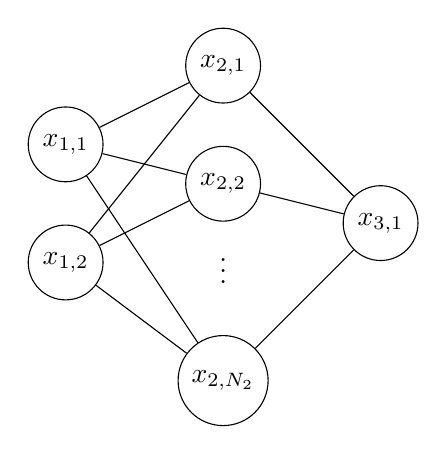
\begin{tikzpicture}
    \tikzstyle{neuron}=[draw,circle];
    \node (x11) [neuron] at (-2,1.5) {$x_{1,1}$};
    \node (x12) [neuron] at (-2,0) {$x_{1,2}$};
    \node [neuron] (x21) at (0,2.5) {$x_{2,1}$};
    \node [neuron] (x22) at (0,1) {$x_{2,2}$};
    \node (x23) [neuron] at (0,-1.5) {$x_{2,N_2}$};
    \node (x31) [neuron] at (2,0.5) {$x_{3,1}$};
    \node at (0,0) {$\vdots$};
    
    \foreach \i in {1,2}{
        \foreach \j in {1,2,3}{
            \draw (x1\i) -- (x2\j);
        }
    }
    
    \foreach \j in {1,2,3}{
        \foreach \k in {1}{
            \draw (x2\j) -- (x3\k);
        }
    }
    
\end{tikzpicture}
        \caption{网络结构}\label{fig:network}
    \end{figure}

    \subsection{算法小结}

    下面将采用矩阵记号简化运算,以下 $\times$ 均表示矩阵的逐点相乘。设第 $k-1$ 层的数值矩阵为 $\mathbf{X}_{k-1}=(x_{k-1,i})_{N_{k-1}\times 1}$,其逐项平方矩阵为 $\mathbf{Y}_{k-1}=(x_{k-1,i}^2)_{N_{k-1}\times 1}=\mathbf{X}_{k-1}\times\mathbf{X}_{k-1}$,向后的权重矩阵为 $\mathbf{U}_{k}=(u_{kji})_{N_{k}\times N_{k-1}}$, $\mathbf{V}_{k}=(v_{kji})_{N_{k}\times N_{k-1}}$,偏移量矩阵 $\mathbf{B}_{k}=(b_{kj})_{N_{k}\times 1}$。

    \subsubsection{前向运算}

    公式 \eqref{eq:def} 将被改写为
    \begin{equation*}
        \mathbf{X}_{k} = f\left(\mathbf{U}_{k}\mathbf{Y}_{k-1} + \mathbf{V}_{k}\mathbf{X}_{k-1} + \mathbf{B}_{k}\right)
    \end{equation*}
    为了简单起见,保留中间结果 
    \begin{align}
        \mathbf{N}_{k}&=\mathbf{U}_{k}\mathbf{Y}_{k-1} + \mathbf{V}_{k}\mathbf{X}_{k-1} + \mathbf{B}_{k}\\
        \mathbf{X}_{k}&=f(\mathbf{N}_k)
    \end{align}

    \subsubsection{后向运算}

    令 $\mathbf{D}_M$ 为目标输出矩阵,将公式 \eqref{eq:outlocalgrad} 改写,输出层的梯度计算为
    \begin{equation}
        \boldsymbol{\delta}_{M} = (\delta_{M,i})_{N_M\times 1} = (\mathbf{D}_M - \mathbf{X}_M)\times f^\prime(\mathbf{N}_M)
    \end{equation}

    改写公式 \eqref{eq:hiddenlocalgrad},隐含层的梯度计算为
    \begin{equation}
        \boldsymbol{\delta}_{k-1} = \left(\mathbf{U}_{k}^T\boldsymbol{\delta}_{k}\times 2\mathbf{X}_{k-1}+\mathbf{V}_{k}^T\boldsymbol{\delta}_{k}\right)\times f^\prime(\mathbf{N}_{k-1})
    \end{equation}

    改写公式 \eqref{eq:u} 和公式 \eqref{eq:v},权重修正矩阵
    \begin{align*}
        \mathbf{\Delta U}_{k} &= (\Delta u_{kji})_{N_{k}\times N_{k-1}} = \eta_1 \boldsymbol{\delta}_k\mathbf{Y}_{k-1}^T \\
        \mathbf{\Delta V}_{k} &= (\Delta v_{kji})_{N_{k}\times N_{k-1}} = \eta_2 \boldsymbol{\delta}_k\mathbf{X}_{k-1}^T 
    \end{align*}

    改写公式 \eqref{eq:bias},偏移修正矩阵
    \begin{equation*}
        \mathbf{\Delta B}_{k} = (\Delta b_{kj})_{N_{k}\times 1} = \eta_3 \boldsymbol{\delta}_{k}
    \end{equation*}

    \subsection{动量项}

    为了加速收敛过程,对修正项添加动量项
    \begin{align}
        \mathbf{\Delta U}_{k}(t+1) &= \alpha_1\mathbf{\Delta U}_{k}(t) + \eta_1 \boldsymbol{\delta}_k\mathbf{Y}_{k-1}^T \\
        \mathbf{\Delta V}_{k}(t+1) &= \alpha_2\mathbf{\Delta V}_{k}(t) + \eta_2 \boldsymbol{\delta}_k\mathbf{X}_{k-1}^T \\
        \mathbf{\Delta B}_{k}(t+1) &= \alpha_3\mathbf{\Delta B}_{k}(t) + \eta_3 \boldsymbol{\delta}_{k}
    \end{align}
    其中 $\alpha_1,\alpha_2,\alpha_3$ 为动量常数。

    \subsection{训练过程}

    根据 \cite{torchlinear},将参数初始化为 $\mathcal{U}\left(-\sqrt{\frac{1}{2}},\sqrt{\frac{1}{2}}\right)$ 上的随机值,其中 $\mathcal{U}$ 为一致分布。

    简便起见,将三个参数的学习率设置为一个相等的值 $\eta_1=\eta_2=\eta_3=\eta$,将动量常数也设为相同的值 $\alpha_1=\alpha_2=\alpha_3=\alpha$。

    数据范围是 $x\in[-6,6],y\in[-6,6]$。

    \section{分割子问题}

    \begin{problem}
        Divide the problem.
        \begin{enumerate}
            \item Divide the two spirals problem into four or nine sub-problems randomly and with prior knowledge, respectively.
            \item Train MLQP on these sub-problems and construct two min-max modular networks.
            \item Compare training time and decision boundaries of the above two min-max modular networks.
        \end{enumerate}
    \end{problem}

    \bibliography{ref}
\end{document}